% easychair.tex,v 3.5 2017/03/15

\documentclass{easychair}
%\documentclass[EPiC]{easychair}
%\documentclass[EPiCempty]{easychair}
%\documentclass[debug]{easychair}
%\documentclass[verbose]{easychair}
%\documentclass[notimes]{easychair}
%\documentclass[withtimes]{easychair}
%\documentclass[a4paper]{easychair}
%\documentclass[letterpaper]{easychair}

\usepackage{doc}

% Sample optional packages to use
\usepackage{graphicx}
\usepackage{amscd}
\usepackage{amssymb}
\usepackage{epsf}
\usepackage{pgf}
\usepackage{url}
\usepackage{flushend} % to balance references on last page

\usepackage{amsmath,amsfonts}
\usepackage{psfrag}
\usepackage{algorithm}  %for algorithm environment
\usepackage{algpseudocode}
\usepackage{siunitx}
\usepackage{subfig}
\usepackage{pifont}
%\usepackage[amsmath,hyperref,thmmarks]{ntheorem}  %better package for proof environment
\usepackage{cite}
\usepackage{hyperref}
\usepackage[capitalise]{cleveref}
\usepackage{booktabs}
%\usepackage[amsmath,hyperref,thmmarks]{ntheorem}  %better package for proof environment
\usepackage{pgfgantt}
\usepackage{import}
\usepackage[disable]{todonotes}

% use this if you have a long article and want to create an index
% \usepackage{makeidx}

% In order to save space or manage large tables or figures in a
% landcape-like text, you can use the rotating and pdflscape
% packages. Uncomment the desired from the below.
%
% \usepackage{rotating}
% \usepackage{pdflscape}


\graphicspath{{./fig/}}

%\makeindex

%% Front Matter
%%
% Regular title as in the article class.
%
\title{Indirect Visual Odometry with Optical Flow}

% Authors are joined by \and. Their affiliations are given by \inst, which indexes
% into the list defined using \institute
%
\author{
Chenguang Huang 
\and Andong Tan 
}

% Institutes for affiliations are also joined by \and,
\institute{
	Technische Universit\"at M\"unchen, Fakult\"at f\"ur Informatik,
	Lehrstuhl f\"ur Robotik und Echtzeitsysteme,\\
	Boltzmannstra{\ss}e 3, 85748, 
	Garching, Germany.
	\email{chenguang.huang@tum.de}
    \email{andong.tan@tum.de}
 }

%  \authorrunning{} has to be set for the shorter version of the authors' names;
% otherwise a warning will be rendered in the running heads. When processed by
% EasyChair, this command is mandatory: a document without \authorrunning
% will be rejected by EasyChair

\authorrunning{Huang, Tan}

% \titlerunning{} has to be set to either the main title or its shorter
% version for the running heads. When processed by
% EasyChair, this command is mandatory: a document without \titlerunning
% will be rejected by EasyChair
\titlerunning{Indirect Visual Odometry with Optical Flow}

\begin{document}

\maketitle

	\begin{abstract}
		   With the increasing need of robotics application in many different domains like autonomous driving and factory cooperative robots, the navigation becomes an important topic. The camera, at the same time, is nowadays a type of cheap sensor, which is powerful in extracting useful information from visual input. Therefore, vision based navigation turns out to be an effective solution. In vision based navigation, visual odometry is an important module. This paper presents the implementation details of visual odometry using the method of optical flow. The novel point of this implementation is that we segment the image using grids and use the number of empty cells to decide key frames. Besides, we evaluate the influence of this parameter and compare this implementation with another implementation which fully depends on descriptor based key point matching in visual odometry.
		    
	\end{abstract}

% The table of contents below is added for your convenience. Please do not use
% the table of contents if you are preparing your paper for publication in the
% EPiC Series or Kalpa Publications series

\setcounter{tocdepth}{2}
{\small
\tableofcontents}

%\section{To mention}
%
%Processing in EasyChair - number of pages.
%
%Examples of how EasyChair processes papers. Caveats (replacement of EC
%class, errors).

%------------------------------------------------------------------------------

%\input{sections/introduction}
%\input{sections/basic_concept}
%\input{sections/structure_design}
%\input{sections/implementation}
%\input{sections/evaluation}
%\input{sections/conclusion}

%\begin{IEEEkeywords}
%	Optical Flow, Visual Odometry, Computer Vision
%\end{IEEEkeywords}


\section{Introduction}
Computer vision related tasks in robotics are attracting more and more attention. One typical task is the visual odometry. It is used widely in applications which require the depth information of objects without directly relying on distance measurement sensors like Lidar. Besides, many applications uses visual odometry to help with the motion planning of some specific agent. Therefore, this function could cause critical problems if it is not reliable. To ensure the safety of the agent, a common choice is to use mathematically provable methods to realize the function rather than using currently unexplainable techniques like deep learning. Thus it worths looking into the implementation details of visual odometry using traditional explainable methods.

To estimate the depth of some specific object, at least two images are needed if there is no prior assumption in how the world is constructed. However, before estimating the depth through triangulation, corresponding point in two images which describes the same 3D point should be found. The first way to achieve this is through key point detection in both images, and find the matching point pairs through similarity comparison. The second way to achieve this is through optical flow, which computes an estimated position of a pixel in the second image according its position in the first image. The above two ways are also suitable to find the point matching pairs between consecutive frames. 

This paper mainly compares the above two methods. 

The following sections are structured as below: Section II presents some basic concepts used in the two methods. Section III describes the pipeline of the two methods. Section IV shows the implementation details. Section V evaluates the difference between these two methods, and Section VI concludes the work.


\section{Basic Concepts}
To understand the methods better, some basic concepts are summarized in this section.

\subsection{Visual Odometry}
Odometry means the estimation of the change in position over time. And visual odometry refers to the estimation of the motion of a camera in real time through sequential images. In the context of vision based navigation, where cameras are often integrated in the robot, visual odometry can be used to estimate the ego motion of the mobile robot, and thus help to build a map in real time around the robot to support the navigation.

\subsection{Optical Flow} The optical flow is apparent 2D motion which is observable between consecutive images. It can also be understood as pixel-wise motion estimation, because the optical flow calculates the motion of a specific pixel between two consecutive frames. Two main types of optical flow calculation are the Lukas \& Kanade method (indirect method) and Horn \& Schunck method (variational method). These two methods have different assumptions but both calculates the optical flow through an optimization process.

In Lukas \& Kanade method, it assumes that (i) the motion is constant in a local neighborhood (ii) the brightness of a specific pixel is constant in different frames. Under the above assumptions, the energy function in the Lukas \& Kanade method is formulated as follows:

\begin{equation}
E(v) = \int_{W(x)} |\Delta I(x', t)^Tv + I_t(x',t) |^2dx'
\end{equation}

where $I(x',t)$ denotes the brightness of position $x'$ at time $t$ in the image, $I_t$ denotes the derivative of brightness with respect to the time $t$, and $W(x)$ denotes the neighborhood of pixel $x'$. The optical flow $v$ is calculated via the minimization of the above energy function. It generates sparse flow vectors.

In contrast, the Horn \& Schunck method assumes (i) the brightness of a specific pixel is a constant in different frames (ii) the motions are spatially smooth. This method generates dense flow vectors. The energy function of this method is:

\begin{equation}
E(u,v) = \int\int[(I_xu + I_yv + I_t)^2+\alpha^2(||\Delta u ||^2 + ||\Delta v ||^2)]dxdy
\end{equation} 

where $I_x$ and $T_y$ are the derivatives of brightness with respect to x and y axis, respectively. $u$ and $v$ are velocity in vertical and parallel directions. In the end, optical flow is obtained through solving for $u$ and $v$ variable.		

\subsection{Key Point Detection}
The environment is continuous and complex. To successfully navigate in such en environment, some key information is more important than the other information. In the image, one kind of typical key information is the corner point. 

One usual method to detect such corner points is through the analysis of the gradient of the image \cite{gradient}. Typical methods include Foerstner and Harris detector \cite{detector}. More recently, detectors like BRIEF, SURF, FAST, and Shi-Tomasi are quite popular, and have many extended versions. In our experiment, key point detection is used to extract important information from the image frames to build the map.

\subsection{Point Matching}
To construct a 3D map, the matching relationship of points between frames are important, otherwise it will cause big error in the triangulation and possibly make the optimization process in determining the 3D position of a landmark unable to converge.

Finding matches between point in consecutive frames are typically done through the comparison of descriptors of two points. If the similarity between two descriptors is high enough, the two corresponding points are considered to be different projections of the same real world point. 

One method to compute the descriptor is called the ORB descriptor \cite{orb}. ORB descriptor uses the BRIEF descriptor \cite{brief} and the orientation of the detected key points to represent the feature of a corner point. According to a set of principles, the correspondence of points between frames will be calculated.

\section{Structure Design}
%(finished)我感觉这里不能默认读者已经知道了exercise 5 在干什么,直接说our pipelie is different in 3cases. 不然paper看起来很奇怪,还是得大概介绍一下区别 


Our pipeline assumes that the stereo cameras have already been calibrated, which means intrinsic matrix and relative transformation between two camera are already known. To make the pipeline easy to understand, we will demonstrate our pipeline in three different conditions: first key frame, second or later key frames and non-keyframes. The criteria of deciding whether a certain frame is key frame will also be discussed later.

\subsection{First key frame}
If this frame is key frame and the first frame, we firstly use Shi-Tomasi method to detect key points in the left image and use optical flow to acquire the corresponding key points in the right image. To increase the correctness of the result of optical flow, we perform optical flow backward and see whether the result key points are adequately close to input key points in the left image. Moreover, to filter out more outliers, we use the relative transformation acquired from calibration to calculate the essential matrix and perform epipolar constraint check. In the next step, we localize the camera by initializing the first pose of left camera with identity matrix. Finally, we use triangulation rule to calculate landmarks, the 3 dimensional position of key points in world coordinate frame. 

\subsection{Second or later key frames}
If this frame is key frame and the second or later frame, we firstly use optical flow to acquire corresponding key points from last left image to current left image. Also a backward check is performed. Later we make a grid on the current left image and detect empty cells in the grid which do not contain key points. In the next step, we use Shi-Tomasi method to detect new key points inside these empty cells. In this period, we have two kinds of key points in the left image. One type includes key points acquired with optical flow from last frame, which we will call old key points. The other type includes newly detected key points with Shi-Tomasi method in empty cells, which we will call new key points. Given these key points in the left image, we perform optical flow from left image to right image and backward check. And then we use epipolar constraint to find inliers. Later on we use RANSAC to localize camera with only inliers of old key points in the left image. Finally we use triangulation to calculate new landmarks with new key points and add observations of old key points to old landmarks.

\subsection{Non-keyframes}
If this frame is not key frame, we firstly perform frame to frame optical flow and make grid as in the second case above. But instead of detecting key points in empty cells, here we only count the number of empty cells which we will use as one of key frame determination criteria. Later we localize camera with RANSAC.\\

Basically the pipeline of three circumstances is shown in the Figure \ref{fig:pipeline structure}.

\begin{figure}[h!]
	\centering
	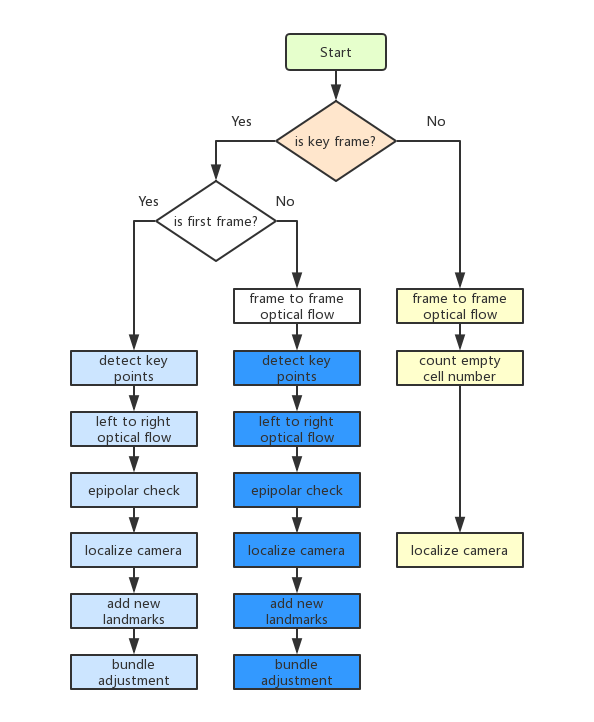
\includegraphics[width=0.7\textwidth]{img/flowchart.png}
	\caption{Pipeline structure}
	\label{fig:pipeline structure}
\end{figure}



\section{Strategies}
This section describes the implementation details of indirect visual odometry with optical flow. As the main difference between optical flow based method and fully key point descriptor matching based method is in the key point matching process and key frame choosing process, these two aspects are highlighted in the rest of this section.

%(finished)另外最好有一个关于optical flow 怎么实现的段落?比如我们调了opencv 的包,用了0.01的参数,之类的?毕竟标题是visual odometry with optical flow, 一直没有提optical flow 怎么实现的,implementaion里应该提一下



\subsection{Key Framing Strategies}
The criteria of key framing is of significant importance. It will affect the accuracy and efficiency of our algorithm1. On the one hand, if one frame can be easily regarded as a key frame, the interval between key frames will become very small. So the optimization will be limited in a small range, focusing too much on local features instead of a global view. In the meantime, more key frames means more optimization time, which makes the algorithm inefficient. On the other hand, if the key framing criterion is too strict so that only very few frames can be selected as key frames, the pipeline is more likely to collapse during the run. This is because we only detect new key points in key frames and if the interval between key frames is too big, the base line will be too large for optical flow to find correspondences through all the frames. Once there are not enough correspondences, the camera localization will become very unstable and the algorithm will fail.\\

In our pipeline we use two criteria to decide whether next frame is key frame. The first criterion is the number of inliers. One necessary step in each time frame is the camera localization. By using RANSAC method, a certain number of inliers are selected for determining the pose of camera. To guarantee there are enough key points for localization, we set a threshold for the number of inliers. If the number of inliers is lower than the threshold, we will treat next frame as key frame. The second criterion is the number of empty cells. As stated in above section, for every non-keyframe a grid is made on the image recorded by the left camera and the number of empty cells will be recorded. A large empty cells number means the feature points calculated by optical flow gather in a small area of the image, indicating that the existing landmarks are leaving observation view. Once the empty cells number exceeds a threshold, we must set the next frame as key frame to detect new key points. In this way, the key points in the image will be adjusted from time to time to distribute relatively uniformly, making localization more stable.

\begin{figure}[h!]
\centering
\subfloat[detect in subimage]{
\begin{minipage}[t]{0.49\textwidth}
\centering	
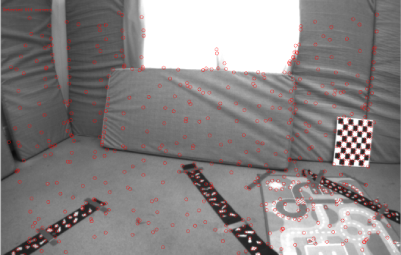
\includegraphics[width=1\textwidth]{img/subimage_keypoint_detection_129.png}	
	
\end{minipage}
}
\subfloat[detect in whole image]{
\begin{minipage}[t]{0.491\textwidth}
\centering	
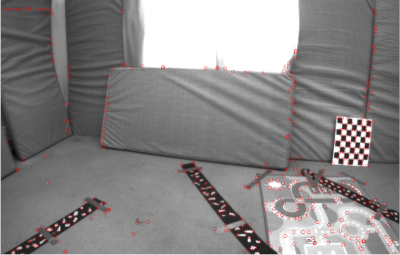
\includegraphics[width=1\textwidth]{img/whole_image_keypoints_detection_129.png}

\end{minipage}
}
\caption{key points detection strategies}
\end{figure}



\subsection{Key Points Detection Strategies}
In every key frame, we have to detect key points in empty cells. We try two different implementations of key points detection in our pipeline. In the first method, we detect key points in the whole image, choose the best key points (max. 1500) and then only keep key points in empty cells. In the second method, we extract empty cells as a series of subimages and detect the best one key point (if at least one key point is detected) in each sub-image separately. %The maximum limit key points detection in the first method is set to 1500 per image. In the second method, it is set to 1 per subimage. 
The difference between these two key point detection methods is shown in Figure \ref{fig:subimage} and Figure \ref{fig:whole image}. We can easily see that the number of detected key points in the second method is larger than the first method. More importantly, the distribution of key points in the second method is more uniform. To quantify the influence of key point detection methods, we run the whole pipeline on euroc dataset and compare the root mean square error of camera trajectories. Finally, we find that the second method performs slightly better than the first method.




\section{Implementation}
\subsection{Lucas and Kanade optical flow with OpenCV}
To track the key points between different frames, we implement three functions: \emph{OpticalFlowBetweenFrame\_opencv\_version}, \emph{OpticalFlowToRightFrame\_opencv\_version} and \emph{OpticalFlowFirstStereoPair\_opencv\_version}. All of these three function needs to input one source image, one target image, source key points data and target key points data. For the algorithm of optical flow, we use the Lucas and Kanade method implemented in OpenCV and use patch window size (21 x 21) and pyramid level 4. A backward optical flow is also performed to improve the robustness of tracking. Only when the distance between the backward result point and its corresponding input point is smaller than 1 pixel can the tracking result be regarded as valid. \\

Among these three functions, the difference lies in the correspondence map they establish. In \emph{OpticalFlowBetweenFrame\_opencv\_version}, we establish match data that match feature ID and track ID. In this way, the key points in current frame can have correspondence with key points of existing landmarks. In \emph{OpticalFlowToRightFrame\_opencv\_version}, we establish match between key points in the left and right images. Furthermore, we have to distinguish whether the optical flow result key points in the right image are from old key points or from newly detected key points. So we use two match data, one for matching between old key points in the left image and their resulting key points in the right image, one for newly detected key points in the left image and their correspondence in the right image. In \emph{OpticalFlowFirstStereoPair\_opencv\_version}, we only create stereo match data. Because this function is for stereo track in the first time step, we do not need to distinguish whether the key points are new or old.

\subsection{Illumination invariant optical flow with manual implementation}


\subsection{Cell and grid}
In order to make cells more conveniently, we implement a class to represent a single cell and a function to make grid on image. \emph{Cell} is a class which contain the coordinates of four corners of a cell and also the key points number inside this cell. By using function \emph{makeCells}, we can create a vector of \emph{Cell}s and initialize the key points number in each cell with 0. \emph{makeCell} needs to input the width and height of an image, how many rows and columns of cells, and a vector used to store cells. To modify the rows number and columns number easily, we set global variables \emph{rnum} and \emph{cnum} at the beginning of \emph{odometry.cpp} for tuning.\\

In order to determine whether next frame is a key frame, one option is to judge whether the empty cells number exceeds a certain threshold. We also implement a function, \emph{check\_num\_points\_in\_cells}, which can update the number of key points in a vector of cells when key points and the cells vector are provided.  \emph{sparsity} function return the empty cells number and their indices when a vector of cells is given. \\

\subsection{Key points detection}
We implement two version of key points detection function. They use different strategies as stated in strategy section above. \\

\emph{add\_new\_keypoints\_from\_empty\_cells} detects key points in each subimage. By inputing the cells vector, empty cells indices and image on which key points will be detected, the function extracts subimage specified by each empty cell and perform Shi-Tomasi key points detection algorithm on that subimage. There is some details we need to pay attention to. First, the detected key points coordinates are relative to the subimage, so we need to add the coordinate of top left corner of the subimage to the result to acquire the position of key points in the whole image. Second, considering that optical flow algorithm uses patch around key points for tracking, we ignore the key points detected in the boundary subimage to ensure the patches can entirely lie in the whole image. Third, the maximum key points number in each subimage is set to 1.\\

\emph{add\_new\_keypoints\_from\_empty\_cells\_v2} detects key points in whole image and then delete the key points in non-empty cells. The maximum key points number is also input to the function.\\

\section{Evaluation}
This section evaluates the performance difference between the matching method using optical flow and the matching method fully relying on key point detection, as well as the performance of the optical flow method under different set of hyper parameters. The evaluation focuses on three main aspects: precision, execution time, and visualization.

As described in the previous section, we use a grid to segment the image frame and decide whether the next frame is a key frame. A basic set of parameters for the grid of our experiments are as follows:


\begin{table}[h!]
	\begin{center}
		\caption{\textbf{Basic set of parameters (unit: pixel)}}
		\label{tab:basicset}
		\begin{tabular}{llll} % <-- Alignments: 1st column left, 2nd middle and 3rd right, with vertical lines in between
			Image height & Image width & Grid size& Min. num. of key points\\
			$h (pixel)$ & $w (pixel)$ & $s (pixel\times pixel)$ & $m$ \\
			\hline
			480 & 752 & 32 $\times$ 32 & 100 \\
			
		\end{tabular}
	\end{center}
\end{table}

The grid size is designed to be so such that it's divisible by the image height and width. Besides, we find through experiments that square grids brings higher precision in the following experiments than rectangular grids. Similarly, the minimum number of key points 100 is found through experiments. To simplify the following discussion, we set the grid size and the minimum number of key points to be a constant, and discuss the influence of other hyper parameters in the rest of the section.
%%
%\itemize
%\item  Strategy

%1. Square grid

%2. Add key points in each cell

%3. Use empty cells number to decide next key frame
%%

\subsection{Precision}

\begin{table}
	\centering
	\caption{\textbf{RMSE precision under different number of Max. empty cells}}
	\label{tab:precision}
	\begin{tabular}{llllll}
		Max. number of \\empty cells (\%)  & 0.35 & 0.4 & 0.42 & 0.44& 0.46 \begin{tabular}[c]{@{}l@{}}  \\\end{tabular}  \\ \hline
		RMSE  & 0.1303 & 0.1295 & 0.1099&0.1563&0.1304\\
		& & & & &\\ 
		Rmse using method \\without optical flow:&0.1012 & & & &		                                                
	\end{tabular}
\end{table}

The table \ref{tab:precision} shows how precision measured as Root Mean Square Error (RMSE) changes when the maximum number of empty cells percentage changes. This variable is designed to control the maximum area of the image where there is no key point. When the empty area is too big, it means we losses a lot of information from these areas and our construction of the map could be not precise enough. When this happen, the next frame will be set as a key frame, and key point detection will be executed. 

From the table it is clear that when the maximum number of empty cells percentage is too small or too large, the precision of the built map will decrease. This means, if we do new key points detection too frequently, we would construct the map using too many key points, which means too many noises, as the key point detection itself is also not 100\% precise. However, if we do key point detection too sparsely, we would have too less key points to construct the map, which indicates that even some small noises could cause a big error in map construction and thus cause an increased RMSE value. In the best case, the RMSE will reach a similar value as the method without using optical flow. Figure \ref{fig:max_empty_cell} shows more experiment data in a visualized way.

\begin{figure}
	\label{fig:max_empty_cell}
	\centering
	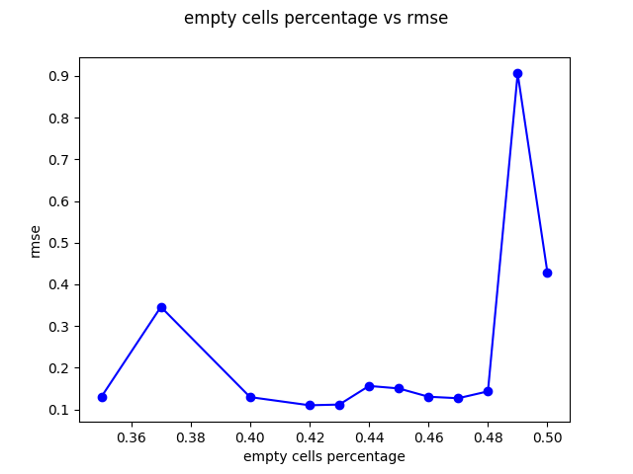
\includegraphics[width=0.7\textwidth]{img/max_num_empty_cell1.png}
	\caption{Visualized version of RMSE change with different parameter of max. number of empty cells percentage}
\end{figure}


\subsection{Execution Time}
The evaluation on execution time includes three parts: detection time, optimization time, and key point matching time. Choosing these three aspects is because: all these three steps are common in two methods, and the difference between these two methods has a big impact on the execution time of these three steps.

%Because the two methods mainly differ in key point detection process, %which influences the optimization time a lot, and the optical flow %method has additionally the optical flow calculation time. Besides, the %optimization step also takes most of the time in the whole %Simultaneously Localization And Mapping (SLAM) process. 

\subsubsection{Detection Time}
The table \ref{tab:detection} shows how detection time changes with change of max number of empty cells percentage. Firstly, it is obvious that the detection time in the method using optical flow is much less than the method without optical flow, because the method using optical flow has replaced a lot of key point detection operation and find the matching points between frames using optical flow. Secondly, it's reasonable to see that with an increasing threshold for maximum empty cells percentage, the detection time generally decreases. This is due to the decreasing frequency of key frames, therefore the detection operation is executed less frequently. The experiment result shows that there is a slight increase on detection time when the threshold is set to 0.44 in comparison to 0.42, we think this could due to the fact that some frames have more textures and corners than the others, and a specific choice of 0.44 occasionally lets us have more key frames in these pictures with a lot of texture and corners. And thus increases the detection time slightly.  

\begin{table}
	\centering
	\caption{\textbf{Detection time under different number of Max. empty cells percentage}}
	\label{tab:detection}
	\begin{tabular}{llllll}
		Max. number of \\empty cells (\%)  & 0.35 & 0.4 & 0.42 & 0.44& 0.46 \begin{tabular}[c]{@{}l@{}}  \\\end{tabular}  \\ \hline
		Detection time (s)  & 3.03643
		& 2.73232
		& 2.43286&2.62328&2.26326\\
		& & & & &\\
		Detection time using method \\without optical flow: &44.0214 & & & &		                                                
	\end{tabular}
\end{table}


\begin{table}[b]
	\centering
	\caption{\textbf{Optimization time comparison}}
	\label{tab:optimization}
	\begin{tabular}{lll}
		& Max. number of empty cells(\%) = 0.42 & Method without optical flow   \\ \hline
		Opt. time (s)  & 305.043 & 65.8619\\
		Num. landmarks &290657 &221886\\
		Num. observation & 1939460 & 559563 \\        
		Num. key frames & 414 & 170                 
	\end{tabular}
\end{table}

\subsubsection{Optimization time}
Optimization takes the most time of the whole pipeline. Here we choose the best parameter for maximum percentage of the number of empty cells, which is 0.42 and compare it with the method without optical flow. The results are shown in table \ref{tab:optimization}.

The optimization time of the optical flow method is much higher than the method fully depending on key point detection. Although the number of landmarks are in similar level, the number of key frames and observation in optical flow method is much higher than the other one, which causes the huge difference in optimization time. As the optimization process only happen in key frames, an increased number of key frames naturally increases the total optimization time. Here comes automatically the question: Why do we have more key frames and observations in optical flow based method?

Firstly, selection of key frames based on counting empty cells (optical flow method) rather than key point number (non optical flow method) in the image leads to a denser choice of key frames. Therefore the number of key frames is much higher.

Secondly, a possible reason for the large number of observations is that our pipeline forces a key point detection operation in every small grid of key frames. Although this has the advantage that the detected key points are more widely distributed in the whole image to help with a preciser optimization process, it has the disadvantage that many noises are also introduced and many noisy points are considered as an observation of some specific landmark.  

The above reasons together leads to the difference in optimization time between two methods.



\subsubsection{Key Point Matching Time}
As a replacement of point descriptor comparison between frames, optical flow is used to track the key point between frames. Therefore, we compare the execution time of optical flow and key point matching through descriptors in the following table \ref{tab:matching}:

\begin{table}
	\centering
	\caption{\textbf{Key point matching time comparison}}
	\label{tab:matching}
	\begin{tabular}{ll}
		Point descriptor matching time (s): &5.79\\
		Optical flow calculation (s): & 117.4~143.1   \\              
	\end{tabular}
\end{table}

The optical flow calculation time is much higher than the key point matching using descriptors. This is due to the fact that optical flow calculation includes an optimization process and the result is calculated iteratively, but descriptor comparison is a rather direct method which only needs several basic mathematical operations. Besides, the descriptor used (ORB) is itself also a very efficient and quick method for comparison.

\begin{figure}[h!]
\centering
\subfloat[Optical flow]{
\label{fig:optical_flow_global}
\begin{minipage}[t]{0.49\textwidth}
	
	\centering
	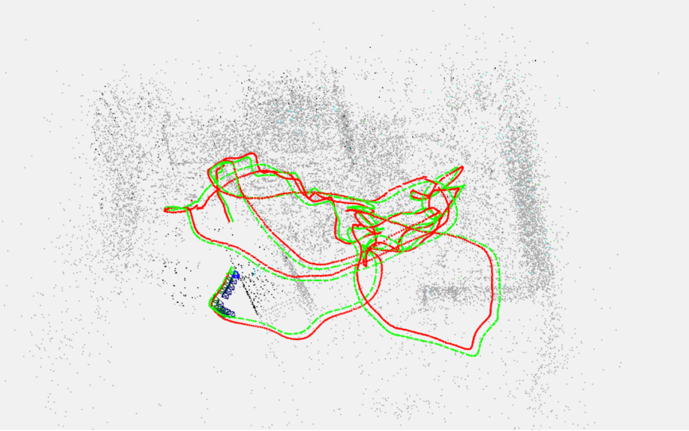
\includegraphics[height=0.6\textwidth]{img/optical_flow_global.png}

	
\end{minipage}
}
\subfloat[Descriptors matching]{
\label{fig:key_point_global}
\begin{minipage}[t]{0.49\textwidth}

	\centering
	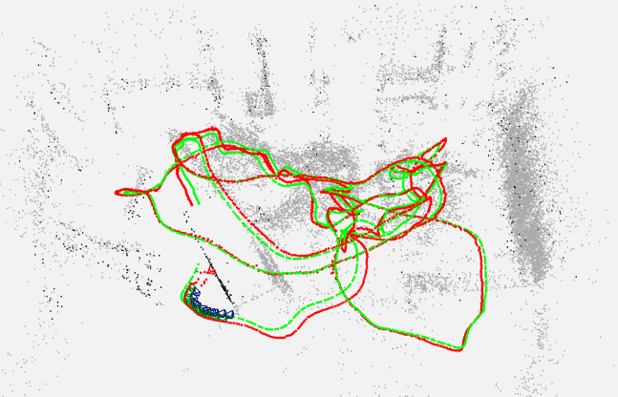
\includegraphics[height=0.6\textwidth]{img/key_point_global.png}
\end{minipage}
}
\caption{Ground truth path (red) and calculated path (green) using optical flow and descriptor matching methods. Gray points represent detected key points.}
\end{figure}

\subsection{Visualization}
A visual comparison can give more intuition for the performance of different methods. 

Comparing the Figure \ref{fig:optical_flow_global} and Figure \ref{fig:key_point_global}, we could find that the detected points using method of optical flow are more uniformly distributed, this is because in the implementation, we force each grid cell of the segmented image to find feature points, which helps to increase the precision of the estimated camera position.

In Figure \ref{fig:optical_flow_desk} and Figure \ref{fig:key_point_desk}, there are two gray lines representing the calibration board in the vertical direction. We could find that the two gray lines in Figure \ref{fig:optical_flow_desk} are closer than Figure \ref{fig:key_point_desk}, which means a better reconstructed map in this area. A real world picture of this area is offered in Figure \ref{fig:desk}.





\begin{figure}[h!]
\centering
\subfloat[Optical flow]{
\label{fig:optical_flow_desk}
\begin{minipage}[t]{0.49\textwidth}
	\centering
	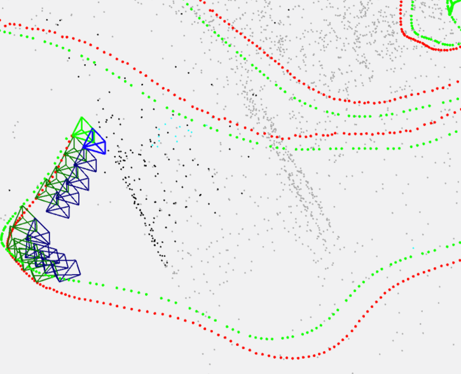
\includegraphics[height=0.7\textwidth]{img/optical_flow_desk.png}	
\end{minipage}
}
\subfloat[Descriptors matching]{
\label{fig:key_point_desk}
\begin{minipage}[t]{0.49\textwidth}
	\centering
	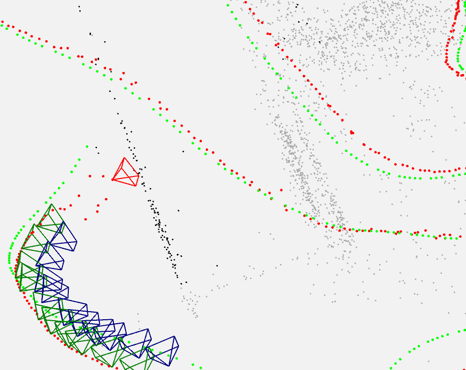
\includegraphics[height=0.7\textwidth]{img/key_point_desk.png}
\end{minipage}
}
\caption{Map constructed using optical flow or descriptor matching. Gray points represent detected key points.}
\end{figure}

\begin{figure}
	\centering
	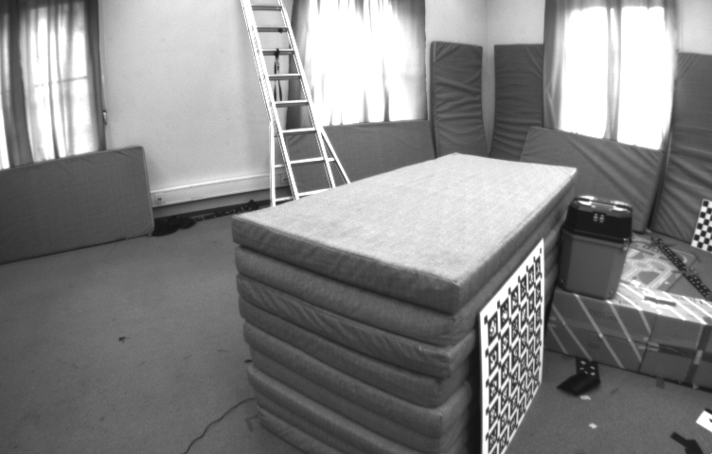
\includegraphics[width=0.5\textwidth]{img/desk.png}
	\caption{The desk image in real world.}
	\label{fig:desk}
\end{figure}




\section{Conclusion}
Visual odometry is a very promising research direction, the applications of this technique is very useful in corresponding environment.

This paper reviews some basic concepts in visual odometry, shows the implementation design and details for visual odometry. Specifically, it presents a novel criterion, which is segmenting image into sub-images and counting number of empty cells to choose key frames. The maximum number of empty cells is a parameter that highly influences the performance of the map construction. A too high or too low number will cause decrease in performance, which indicates that the number of key frames should be kept in a suitable number for a good performance. The strategy of key point detection according to sub-images offers more uniformly distributed key points than key point detection according to the whole image. The execution time is different parts are influenced by the difference between pipeline and the choice of parameter (e.g. max. number of empty cells) in optical flow based implementation.




\begin{thebibliography}{00}
	
	\bibitem{gradient} H. Wang and M. Brady, “Real-time corner detection algorithm for
	motion estimation,” Image and vision computing, vol. 13, no. 9, pp. 695–
	703, 1995.
	
	\bibitem{detector} Rodehorst, V.; Koschan, A. Comparison and evaluation of feature point detectors. In Proceedings
	of 5th International Symposium Turkish-German Joint Geodetic Days, Technical University of
	Berlin, Germany, March, 2006; ISBN 3-9809030-4-4.
	
	\bibitem{orb} E. Rublee, V. Rabaud, K. Konolige, and G. Bradski, “ORB: an efficientalternative  to  SIFT  or  SURF,”  inIEEE  International  Conference  onComputer Vision (ICCV), Barcelona, Spain, November 2011, pp. 2564–2571
	
	\bibitem{brief} E. Rublee, V. Rabaud, K. Konolige and G. Bradski, "ORB: An efficient alternative to SIFT or SURF," 2011 International Conference on Computer Vision, Barcelona, 2011, pp. 2564-2571.

	
	
	
\end{thebibliography}



%\bibliographystyle{plain}
%\bibliographystyle{alpha}
%\bibliographystyle{unsrt}
%\bibliographystyle{abbrv}
%\bibliography{easychair}

\end{document}

